% -*- root: ../../main.tex -*- %

\section{Preliminary decisions} % (fold)
\label{sec:design_decisions}
  All of the variants highlighted in \ref{sub:promising_combinations_of_characteristics} represent possible approaches for the utilization of Docker for the enactment of workflows for different use cases.
  $G_{DV}^{SEPC}$ with a partially integrated workflow engine is the implemented variant for several reasons. First and foremost, this combination enables the use of basic Docker commands for the suspension and continuation of a workflow and single activities, as described in \ref{ssub:element_wrapping_containers}. Second, $*_{*}^{SEPC}$ leverages the already existing communication between the local daemon of a node and the swarm master daemon to publish the status of both workflow instances and activity instances, in the form of events concerning container statuses. Third, $G_{DV}^{*}$ is a promising variant for the demonstration of various scheduling mechanisms introduced in \ref{sub:execution_scheduling}, since this variant includes implicit affinities by default. While partially integrating the workflow engine is mainly interesting for its role in the previously mentioned native pausing, it also facilitates the working directory management, as argued in \ref{ssub:element_wrapping_containers}.

  The services identified in \ref{sub:components} are implemented using \emph{Ruby}, a dynamically typed object-oriented programming language. Ruby provides the means to write concise, well readable code \cite[p.~782]{Nanz2015Comparative}. Performance-wise, it is inferior to many other languages \cite[p.~786]{Nanz2015Comparative}. However, the focus of this thesis is to explore conceptual possibilities rather than developing efficient implementations. An emphasis is thus put on the expressiveness of the used language to help the reader to grasp the underlying concept quickly.

  All services that require access to any Docker \ac{API} use a gem called \texttt{docker-api} which provides a client for these \acp{API}. \emph{Gem} is the name for distributable packages in the Ruby ecosystem. These packages can be managed using \emph{Gemfiles} in which the package dependencies of an application may be declared.

  The Ruby-based web application framework \ac{RoR} is used for the implementation of the developer gateway and user gateway. It qualifies for this task because it comes with several functionalities that aim at the fast creation of prototypes. For example, so called \emph{scaffolds} permit the creation of model and controller classes and appropriate views based on a specified database schema; the included library \emph{ActiveRecord} supports adding object-relational mapping functionality to model classes \cite[p.~5]{Jazayeri2007Some}. ActiveRecord is also used in those services that do not use Rails but need to store objects in databases, namely in the \texttt{definition}, \texttt{organization}, and \texttt{worklist} services.

  PostgreSQL was chosen as database solution for the services, because it supports both relational data, which is useful for storing the models and their relations, as well as the document-store-like JSONB format which allows the schema-less storage of configuration information.

  RabbitMQ was chosen as message oriented middleware, because it is well documented and provides a web interface for monitoring and administration.
  The gems \texttt{Hutch} and \texttt{Bunny} provide different levels of abstraction for the interaction with the RabbitMQ message queue \cite{Software2016Rabbitmq}. \texttt{Hutch} itself is based on \texttt{Bunny} and imposes some opinionated conventions for the use of the message queue, as well as automatic (de-)serialization of the messages' payload.
% section design_decisions (end)

\section{Execution images} % (fold)
\label{sec:execution_images}
  In \ref{sub:workflow_activity_images}, activity images and workflow images are designed. In the following, the implementation of these images is described.

  \begin{figure}[htbp]
    \centering
    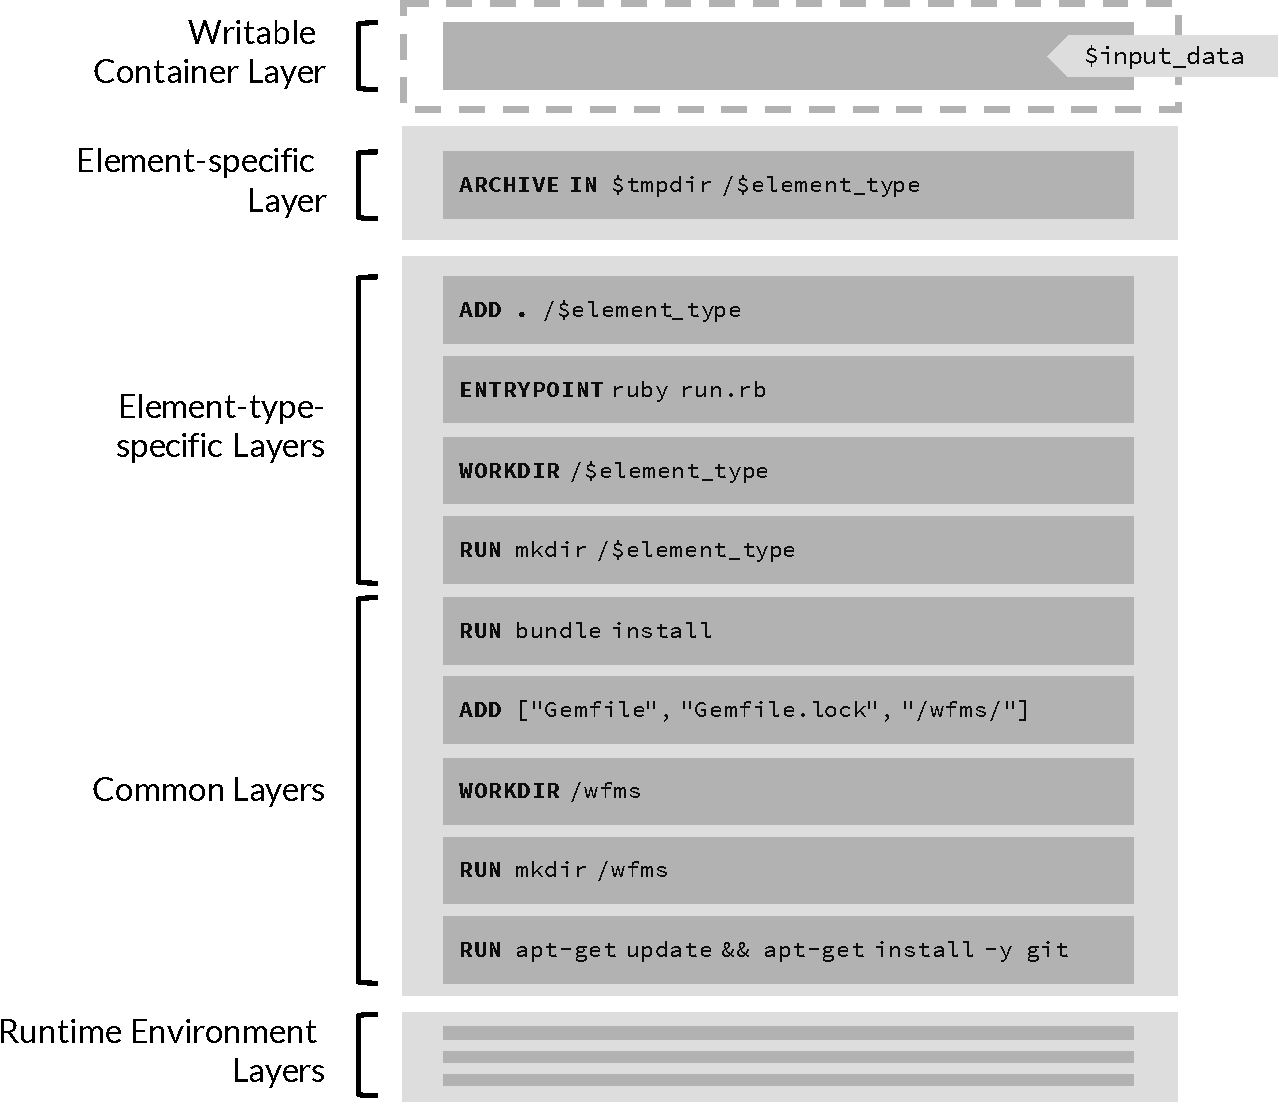
\includegraphics[width=0.95\textwidth]{content/images/execution_container-crop.pdf}
    \caption{Layer Contents for Element-wrapping Containers}
    \label{fig:detailed_layers_for_element_wrapping_containers}
  \end{figure}

  \subsection{Workflow image} % (fold)
  \label{sub:workflow_container}
    The workflow image is implemented as designed in \ref{sub:workflow_activity_images}. The runtime-environment layers are provided by inheriting all layers of the \texttt{ruby:2.2} image. On top of these, common layers are created, in which the required gems are installed. Then, the \texttt{/workflow} directory is created, into which the required Ruby files are copied. The file \texttt{run.rb} is set as the default command.

    The code and the workflow configuration files reside in the \texttt{/workflow} directory. \texttt{pro\-cess\_de\-fi\-ni\-tion.json} contains the exported process definition (Lst.~\ref{lst:exported_process_definition_in_json_format}), \texttt{ workflow.info.json} contains metadata on the workflow (\eg the image name), and \texttt{input.schema.json} contains the \ac{JSON} schema used to validate the workflow instance's input (Lst.~\ref{lst:input_schema_in_json_format}). The instance specific files are copied to \texttt{/workflow} before the container is started.

    As decided in \ref{sec:design_decisions}, the workflow instance features some functionality that one would usually find in a workflow engine. This functionality resides in the \texttt{ProcessInstance} class. On instantiation, the \texttt{ProcessInstance} obtains an instance of the helper classes \texttt{ProcessDefinition} and \texttt{Validator} and instructs the latter to check the validity of the provided input data against the provided \ac{JSON} schema (Lst.~\ref{lst:wf_image_process_instance}~\#4-13). \texttt{ProcessDefinition} parses the process definition file \texttt{process\_definition.json} and makes the contents available as an object (Lst.~\ref{lst:wf_image_process_definition}).

    The \texttt{run} script loads the required dependencies and ensures, that the container is connected to the \texttt{enactment} network. Then, it initiates the enactment by creating an instance of the \texttt{ProcessInstance} class and calling its start method (Lst.~\ref{lst:wf_image_run}).
    When started, \texttt{ProcessInstance} creates a new \texttt{ActivityInstance} for the start activity, creates a symbolic link to the workflow instance's input data, and adds the \texttt{ActivityInstance} to a queue for incomplete activity instances (Lst.~\ref{lst:wf_image_process_instance}~\#16-26). Then, it enters a loop in which it carries out the workflow enactment. It leaves this loop, which calls the method depicted in Listing~\ref{fig:the_processing_loop_of_process_instance} on each iteration, if no more activities are queued for processing.

    \begin{figure}[th]
      \inputminted[firstline=28,lastline=45,fontsize=\footnotesize,linenos=true,numberblanklines=true,showspaces=false,breaklines=true,baselinestretch=1,gobble=2]{ruby}{../code/wf_base/process_instance.rb}
      \caption[The processing loop of ProcessInstance]{The processing loop of \texttt{ProcessInstance}}
      \label{fig:the_processing_loop_of_process_instance}
    \end{figure}

    The called method, \texttt{process\_queued\_activity\_instances}, iterates over the queue of unprocessed activity instances. If the start conditions of such an instance are not met it is skipped for the current iteration. Otherwise, the activity instance is started. As soon as it finishes, an \texttt{ActivityInstance} object is created for each of its succeeding activities. The finished activity instance is added to the successors' lists of completed predecessors, and a symbolic link from its output directory to the respective successor's input directory is created. If the activity was an end activity, a symbolic link is created from its output directory to the workflow's output directory and all pending activity instances are removed from the queue. The loop ends and the workflow instance terminates together with the process instance.

    The actual creation and start of an activity instance container takes place in the \texttt{ActivityInstance} class, which invokes Docker with the command depicted in Listing~\ref{lst:instantiation_of_an_activity_image_in_activityinstance}. The container is named with an instance \ac{ID}, labeled with this very \ac{ID} and also with the \acp{ID} of the directly superordinate workflow instance as well as the overall superordinate workflow instance. The container is based on the suitable activity image and launched without an additional command, as the right command is already specified in the image. To enable the instance container to communicate with the local Docker host, the respective socket is mounted on the container's file system. The data volume that contains the workflow relevant data is bound to the activity instance container, too. Environment variables are set on the container in order to pass along configuration: \texttt{MAIN\_WORKFLOW\_ID}, \texttt{WORKFLOW\_ID}, \texttt{WORKFLOW\_INSTANCE\_ID}, \texttt{ACTIVITY\_ID}, and \texttt{ACTIVITY\_INSTANCE\_ID} are passed to inform the activity instance container about its activity/activity instance \ac{ID} a, as well as the directly superordinate workflow/workflow instance, and finally the \ac{ID}/instance \ac{ID} of the originally called workflow. It is further passed the path of the directory that is designated to be its working directory in the \texttt{WORKDIR} environment variable. The container can then be started using the \texttt{run} command of the \texttt{ActivityInstance} (Lst.~\ref{lst:wf_image_activity_instance} \#27-37).

    \begin{listing}[htbp]
      \inputminted[firstline=40,lastline=68,fontsize=\footnotesize,linenos=true,numberblanklines=true,showspaces=false,breaklines=true,baselinestretch=1,gobble=2]{ruby}{../code/wf_base/activity_instance.rb}
      \caption[Instantiation of an activity image in ActivityInstance]{Instantiation of an activity image in \texttt{ActivityInstance}}
      \label{lst:instantiation_of_an_activity_image_in_activityinstance}
    \end{listing}

  % subsection workflow_container (end)

  \subsection{Activity image} % (fold)
  \label{sub:activity_containers}
    Analogous to the workflow image, the activity image is implemented according to its design in \ref{sub:workflow_activity_images}. Instead of a \texttt{/workflow} directory, the \texttt{/activity} directory is created which contains the necessary code for the activity instance. The file \texttt{run.rb} is set as the default command for the container.

    %The activity image contains the classes \texttt{ActivityInstance}, \texttt{WorklistClient}, \texttt{ContainerInvocation}, \texttt{SubworkflowInvocation}, \texttt{FileHelper}, \texttt{Configuration}, and \texttt{Validator}, as depicted in \ref{fig:uml_class_diagram_activity_image}.
    %\texttt{FileHelper}, \texttt{Configuration}, and \texttt{Validator} have the same functionalities as their counterparts in the workflow image.

    The code and the activity configuration files reside in the \texttt{/activity} directory. These files are \texttt{activity.info.json} and \texttt{input.schema.json}. \texttt{activity.info.json} contains configuration data of the activity, \eg name, version and parameters for a third-party container for a container-type image, or the assigned role for a manual-typed image (Lst.~\ref{lst:activity_info_json}). \texttt{input.schema.json} contains the \ac{JSON} schema that is used to validate the activity instance's input.

    Depending on the activity type, the activity instance either starts a specified third-party container (container activity), a workflow instance container (sub-workflow activity), or issues a worklist item for manual data input (manual activity), by using the \texttt{ContainerInvocation}, \texttt{SubworkflowInvocation}, or \texttt{WorklistClient} classes respectively. The outcome of these actions is then stored in the output data file. For this prototype all other activities, \ie the control flow activities, log the activity and activity instance \acp{ID} to that data file as a proof of their invocation.

    \begin{figure}[htbp]
      \inputminted[firstline=18,lastline=27,fontsize=\footnotesize,linenos=true,numberblanklines=true,showspaces=false,breaklines=true,baselinestretch=1,gobble=2]{ruby}{../code/ac_base/run.rb}
      \caption[]{Instantiation of an activity image in \texttt{ActivityInstance}}
      \label{fig:main_logic_of_ac_instance}
    \end{figure}

    The invocation of another container is performed in the \texttt{ContainerInvocation} class. The container is created based on the specified image and is labeled with the \acp{ID} of the overall superordinate workflow instance, the directly superordinate workflow instance, and the activity instance (Lst.~\ref{lst:container_invocation_helper_class}~\#27-38).
    Once the container's execution has finished, its standard output stream and error output stream can be accessed with the \texttt{results} method (Lst.~\ref{lst:container_invocation_helper_class}~\#18-23). \texttt{SubworkflowInvocation} acts similar to \texttt{ContainerInvocation}, but it uses another configuration for the container -- the same that a workflow engine uses, but with an explicit working directory specified (cf. Lst.~\ref{lst:subworkflow_invocation_helper_class}~\#43-68). A workflow container is thus not aware of whether it is started by a sub-workflow activity or by a workflow engine.

  % subsection activity_containers (end)
% section execution_images (end)

\section{System components} % (fold)
\label{sec:components_implementation}
    In the following, the implementation of the prototype's system components according to the design from  \ref{sub:components} is described.

    Since the principle of event-driven service invocation is already demonstrated in the definition service, a detailed documentation of the organization and worklist services would not contribute further relevant insights. They are thus only described regarding their realization with Docker containers and the network configuration of these containers.

  \subsection{Workflow definition service} % (fold)
    \label{sub:workflow_definition_service}
    The workflow definition service is composed of three components: one container running a Ruby on Rails application which is configured to expose a JSON API, one container running a PostgreSQL database and a data volume container which provides persistent storage to that database (Lst.~\ref{lst:the_whole_docker_compose_file_1}~\#128-148).

    The PostgreSQL database's support for relational data is used for storing the workflow, its elements and their relations. Its capability to store data in the JSONB format is used to store the schema-less storage of configuration information. This is valuable because the structure of those configurations is not known in advance, \eg input validation schemas.
    In order to keep the stored data during container restarts or migrations across nodes, the database makes use of a data volume container which provides its working directory.

    The application container is granted access to the Docker daemon of its host node in form of a mounted volume to build and push images.

    As planned in \ref{subs:workflow_definition_service}, the service has the model classes \texttt{Activity}, \texttt{ControlFlow}, \texttt{ProcessDefinition} and \texttt{Workflow}, which act as object-relational mappers for persistence to the database as well as ensure some validity constraints. Further, there exists a controller class for each of the aforementioned models, which provides \ac{CRUD} actions for the respective model. The \texttt{Activity} model provides the means to store the \acp{ID} of an assigned role, a referenced sub-workflow, validation schemas, and a configuration for a third-party container (Lst.~\ref{lst:activity}~\#8-13). In order to have more fine-grained control over the serialization of a workflow, the \texttt{WorkflowFullSerializer} is used if a specific workflow is requested. It nests all relevant workflow elements into the workflow model before it is serialized (Lst.~\ref{lst:workflow_full_serializer}).

    While the modeling logic is contained in the model and controller classes and in the underlying data schema, the export logic resides in the classes \texttt{ImageManager} and \texttt{ImageBuilder}, which are supported by the class \texttt{ProcessDefinitionImageSerializer}.

    The \texttt{ProcessDefinitionImageSerializer} provides the means to create the consolidated JSON representation of a process definition with all information that is necessary to execute the corresponding workflow. An example for the serialized output can be seen in Listing~\ref{lst:exported_process_definition_in_json_format}.

    Whenever the user requests the export of a workflow, the request is forwarded to the \texttt{ImageManager} (Lst.~\ref{lst:image_manager}).
    In order to export a workflow, the first step is to identify all of its elements that require to be wrapped in an image. Obviously, one of them is the workflow itself. The other required images are determined by traversing the workflow's process definition recursively (Lst.~\ref{lst:activity}~\#37-43, Lst.~\ref{lst:workflow}~\#11-13). Each of the workflow's activities has to be exported. Each sub-workflow has a method that exposes the Docker images it requires beyond that. It does so by passing the call for required images on to the referenced workflow -- which collects its required images analogously -- and returning the result. The \texttt{ImageBuilder} then iterates over all these elements and creates a corresponding image for each (Lst.~\ref{lst:image_builder}~\#6-28). Starting with the respective base image -- \texttt{ac\_base} or \texttt{wf\_base} -- it adds additional layers to do so. The \texttt{ImageBuilder} creates the files which are specific to the current element from the activity's or workflow's configuration, \ie the input/output validation schemas, the element's description file, and in case of a workflow the serialized process definition, in a temporary directory. The \texttt{ImageBuilder} then copies these files to the image and names it after the workflow element that it represents (Lst.~\ref{lst:image_builder}~\#32-95). The \texttt{ImageManager} then uploads all images that were successfully built to the private registry.
    % subsection workflow_definition_service (end)

  \subsection{Organization management service and worklist service} % (fold)
    \label{sub:organization_management_service}
      As envisioned in \ref{sub:components}, the organization management service and the the worklist service are structured analogously to the workflow definition service. Just like it, the services consist of three Docker containers: an application that is backed by a PostgreSQL database that is persisted to a data volume (Lst.~\ref{lst:the_whole_docker_compose_file_1}~\#52-126). They respond to \ac{CRUD} requests which they receive through consumer classes that accompany each of their model classes.
    % subsection organization_management_service (end)

  \subsection{Workflow engine service} % (fold)
    \label{sub:workflow_engine_service}
    As it does not require any data persistence in the chosen setup, the workflow engine service only consists of an application container. The consumer classes \texttt{WorkflowConsumer} and \texttt{WorkflowInstanceConsumer} listen to events that concern the corresponding element types and instruct the \texttt{WorkflowEngine} to perform the according action. The \texttt{DockerHelper} class provides the connection to the swarm master that is used to manage the workflow instances.
    The \texttt{WorkflowInstance} class takes care of the actual instantiation of a workflow and the required preparations that come along with it.

    The \texttt{WorkflowEngine} can pause, unpause or terminate a workflow instance, by querying the swarm master for all containers which bear a label with the workflow instance's \ac{ID}, and then calling the command \texttt{pause}, \texttt{unpause}, or both \texttt{kill} and \texttt{delete} on each of them (Lst.~\ref{lst:wf_engine_class_in_workflow_engine_service} \#26-44).

    \texttt{WorkflowInstance} begins with the enactment of a workflow by creating the data container, which is used later to store the workflow data. The data container is based on the image \texttt{cogniteev/echo}, a small image that provides a single executable -- \texttt{echo} -- because Docker expects one executable to be present in a container \cite{Cogniteev2015Docker}. The container's name is configured to equal the workflow instance's \ac{ID} with the prefix \texttt{data\_} and the \ac{ID} is also passed to the container as value for a \texttt{main\_workflow\_instance} label (Lst.~\ref{lst:workflow_instance_class_in_workflow_engine_service}~\#40-51).
    To show some of the scheduling possibilities, a randomly drawn constraint of the following
    \mint{ruby}{"constraint:edu.proto.machine_env==external"}
    \mint{ruby}{"constraint:edu.proto.ram==/(\d\d\d\d+|[7-9]\d\d|[6][5-9]\d)/"}
    is passed, such that the data container is either scheduled on a external node or a node with at least 650MB of memory (Lst.~\ref{lst:workflow_instance_class_in_workflow_engine_service}~\#49). Each node on which workflows are executed obtains a directory \texttt{/workflow\_relevant\_data}, in which the working directories for the various workflow instances are kept. \texttt{WorkflowInstance} passes the instruction
    \mint{ruby}|"/workflow_relevant_data/#{@instance_id}:/workflow_relevant_data"|
    to create a such a working directory under the name of the workflow instance \ac{ID} and to make it available in the data container at the path \texttt{/workflow\_relevant\_data} (Lst.~\ref{lst:workflow_instance_class_in_workflow_engine_service}~\#48).

    Then, \texttt{WorkflowInstance} resolves the appropriate image name from the workflow's \ac{ID} and creates the workflow instance container -- but it does not start it yet. The container's name is configured to equal the workflow instance's \ac{ID} with the prefix \texttt{wfi\_}. The container is labeled with the workflow instance's \ac{ID} as value for both \texttt{main\_workflow\_instance} and \texttt{main\_workflow\_instance}. \texttt{WorkflowInstance} passes the instructions to mount both the local Docker daemon's socket and the data volume of the previously created data container. The passed affinity
    \mint{ruby}|"affinity:container==#{@data_container.id}"|
    instructs the swarm master to create the container on the same node as the data container. Since the workflow instance is the root of the enactment's instance hierarchy, its workflow and workflow instance \acp{ID} are passed to the container as the values of the environment variables that inform the workflow instance about the superordinate workflow and its instance as well as its own and its workflow's \ac{ID} (Lst.~\ref{lst:workflow_instance_class_in_workflow_engine_service}~\#76-99).

    When instructed to start the workflow instance container, \texttt{WorkflowInstance} connects the container to the \texttt{wfms\_enactment} network, copies the input data into the container, starts it and waits for it to stop.
    Then, it copies out the output \ac{JSON} file, parses and returns its content as an Ruby object to the engine. In a non-prototypical implementation, the containers would be deleted at this point -- in this prototype, they are left on the node for inspection (Lst.~\ref{lst:workflow_instance_class_in_workflow_engine_service}~\#14-29, \#40-60).
    % subsection workflow_engine_service (end)

  \subsection{Developer gateway} % (fold)
    \label{sub:developer_gateway}
    The developer gateway does not require any database, as it merely forwards requests to the services via the \ac{MOM}. Hence, it consists of a single Docker container that contains a \ac{RoR} application. To be reachable by the users, this container needs to expose the port that the \ac{RoR} application is listening on to the host's network (Lst.~\ref{lst:the_whole_docker_compose_file_1}~\#204-218).

    The \ac{RoR} application serves a web interface that offers the means for the inspection of the available nodes, the management of users and roles, and for the modeling of workflows. It does so by sending requests to the application's controllers and presenting the outcome.
    In order to request data from the micro-services, a controller class creates a response queue to which it subscribes. Then it publishes a message on an appropriate queue, in which it declares the need for a specific information. One of the services instances that are subscribed to this queue receives the request and publishes the answer to the respective response queue. The result is then returned to the frontend, where it can be displayed (\eg as in Lst.~\ref{lst:workflows_controller_class_in_developer_gateway}). The required methods are provided by the \texttt{ApplicationController}, from which all other controllers inherit (Lst.~\ref{lst:application_controller_class_in_developer_gateway}~\#24-49).

    % subsection developer_gateway (end)

  \subsection{User gateway} % (fold)
    \label{sub:user_gateway}
    Just like the developer gateway, the user gateway does not require any storage mechanism. It thus also consists of only one Docker container, which contains the \ac{RoR} application. To make the service accessible from outside of the system, the user gateway service's container exposes the port that the  application is listening on the host's network. The user gateway is connected to the frontend network to isolate it from the internal services -- to which it may only communicate through the \ac{MOM}.
    While the backend functionality is implemented in Ruby, the frontend is served by \ac{RoR} as simple \ac{HTML} pages.
    % subsection user_gateway (end)

  \subsection{Message oriented middleware (MOM)} % (fold)
    \label{sub:message_oriented_middleware}
      RabbitMQ exists as a pre-configured Docker image (\texttt{rabbitmq}) on the Docker Hub and can thus put to use swiftly. The configuration of RabbitMQ in this image takes place when the respective container is started which allows its configuration in the \texttt{docker-compose} configuration file as depicted in Listing~\ref{lst:configuration_of_the_mom_service_in_the_docker_compose_file}.
      For the sake of simplicity, no authentication mechanism was introduced besides the simple default username/password combination. As the central point of communication, the \ac{MOM} is the only container which is connected to all three overlay networks. While one would probably avoid exposing this service in a real use case, it is exposed to the host's network for its use in a prototype, as this allows to monitor the messaging activity of the services.

      \begin{listing}[!htbp]
        \inputminted[firstline=23,lastline=33,fontsize=\footnotesize,linenos=true,numberblanklines=true,showspaces=false,breaklines=true,baselinestretch=1]{yaml}{../code/wfms.yml}
        \caption{Configuration of the \ac{MOM} service in the Docker Compose file}
        \label{lst:configuration_of_the_mom_service_in_the_docker_compose_file}
      \end{listing}
    % subsection message_oriented_middleware (end)

  \subsection{Infrastructure management service} % (fold)
    \label{sub:infrastructure_management_service}
      The data this service offers -- the state of the Docker swarm and its nodes -- should always be up-to-date. It is thus gathered ad-hoc when a request arrives. This proceeding makes a database obsolete, that is why the infrastructure management service solely consists of one Docker container which contains the application (Lst.~\ref{lst:the_whole_docker_compose_file_1}~\#170-186).

      The \texttt{EnvironmentManager} queries the Docker daemon to gather the requested information and processes the response (Lst.~\ref{lst:environment_manager_in_infrastructure_managment_service}). It is supported by the \texttt{DockerHelper}, which provides the means to point the local Docker client at arbitrary members of the swarm or the swarm manager.
    % subsection infrastructure_management_service (end)

  \subsection{Registry} % (fold)
    \label{sub:registry}
    A local registry is deployed in its own container in order to distribute the created images.
    Docker provides the \texttt{registry} image for this purpose, of which the version \texttt{registry:2.3} is used, since it is the newest stable version at the time of this writing.

    The registry is configured to be restarted automatically in case that itself or the node it runs on fails. Further, it is exposed on the host's network to make it reachable for all nodes in the swarm. This is necessary as their daemons are not containers and thus cannot be connected to the overlay network. This configuration is reflected in the \ac{WfMS}' Docker Compose file as follows:

    \begin{listing}[!b]
      \inputminted[firstline=12,lastline=21,fontsize=\footnotesize,linenos=true,numberblanklines=true,showspaces=false,breaklines=true,baselinestretch=1]{yaml}{../code/wfms.yml}
      \caption{Configuration of the registry service in the Docker Compose file}
      \label{lst:configuration_of_the_registry_service_in_the_docker_compose_file}
    \end{listing}
    % subsection registry (end)

  \subsection{Provisioning service} % (fold)
    \label{sub:provisioning_service}
      The provisioning service is implemented in a simple way -- it consists of a single script that listens to the events published to the swarm master. If a named image is pushed by one of the nodes, the provisioner pulls its own node, as visible in Listing~\ref{lst:provisioner_loop}.

      \begin{listing}[!t]
        \inputminted[firstline=19,lastline=29,fontsize=\footnotesize,linenos=true,numberblanklines=true,showspaces=false,breaklines=true,baselinestretch=1]{ruby}{../code/provisioner/provisioner.rb}
        \caption{Provisioning service: Loop for pulling images}
        \label{lst:provisioner_loop}
      \end{listing}
    % subsection provisioning_service (end)
% section components (end)


\section{Exemplary deployment and case study} % (fold)
\label{sec:exemplary_deployment}
  To show the feasibility of the developed solution, the prototype is deployed exemplarily. This process is supported by Docker Machine, Docker Swarm, and Docker Compose. Four machines are created to simulate an organization setup (Lst.~\ref{lst:setup_exemplary_deployment_1}). The first machine that is started will serve as a host for the image registry and the key-value store that Docker Swarm uses. It is thus named \texttt{coordination-machine}. To account for the increased need for memory of the registry, this machine receives twice the amount of memory that the other machines will be granted. Three other machines are created, which are equal in their available resources: \texttt{development-machine}, \texttt{internal-machine}, and \texttt{cloud-machine}. The latter is not actually located on a remote location, but its daemon is labeled with
  \\ [0.5ex]
  \centerline{\texttt{edu.proto.machine\_env=external}}
  \\ [0.5ex]
  while the other nodes receive the value \texttt{internal}, to show how such a node could be distinguished for scheduling. Each of the nodes is also labeled with a fictional amount of available memory, \eg
  \\ [0.5ex]
  \centerline{\texttt{edu.proto.ram=1024}.}
  \\ [0.5ex]

  While the allocation of services to specific nodes would not matter in practice, it is done in a static manner for this prototype to facilitate referencing to them during examination and documentation.
  The services are assigned to the nodes as follows: the registry is started on \texttt{coordination-machine}; the \ac{MOM}, worklist, and user gateway services reside on \texttt{internal-machine}; all other services are allocated on \texttt{development-machine}. Creating the registry on the \texttt{coordination-machine} is a good practice, as every Docker daemon that is part of a swarm knows the \ac{IP} address of this machine if the key-value store is also hosted there. Its address can thus be resolved by accessing the daemon's configuration. Further, it may be used to distribute the \ac{WfMS}' images during the installation of the system.

  To recover from service failures, all containers are configured with the option \texttt{restart: on-failure:3}. That is, if a container terminates because of an error, Docker tries to restart it up to three times. While this is not a solution for actual errors in the code, since they will occur again, it may help to recover from failures induced by external factors.

  The deployment of all services is performed using Docker Compose (Lst.~\ref{lst:setup_exemplary_deployment_2}).
  The configuration of all services and the required networks that connect them can be specified in a single \emph{YAML} file. \ac{YAML} is designed with a focus on human readability \cite{Kiki2009Yaml}.
  The configuration file, which is depicted in Listing~\ref{lst:the_whole_docker_compose_file_1}-\ref{lst:the_whole_docker_compose_file_5} can thus serve as a textual documentation of the system's architecture.
  For example, the existence of the three overlay networks determined in \ref{sub:inter_component_communication} is expressed by the lines

  \inputminted[firstline=3,lastline=9,fontsize=\footnotesize,linenos=true,numberblanklines=true,showspaces=false,breaklines=true,baselinestretch=1]{yaml}{../code/wfms.yml}

  and the connection of a container (in this case the workflow engine application container) to these networks is declared as

  \inputminted[firstline=34,lastline=34,fontsize=\footnotesize,linenos=true,numberblanklines=true,showspaces=false,breaklines=true,baselinestretch=1]{yaml}{../code/wfms.yml}
  \inputminted[firstline=43,lastline=45,fontsize=\footnotesize,linenos=true,numberblanklines=true,showspaces=false,breaklines=true,baselinestretch=1]{yaml}{../code/wfms.yml}

  A graphical visualization of the exemplary deployment described by the Docker Compose configuration file is presented in Figure~\ref{fig:deployment_diagram_of_the_architecture}.

  To demonstrate the ability of the prototype to actually operate, an exemplary workflow (\texttt{everything-workflow}) is modeled and executed which consists of two sub-workflow activities: one sub-workflow contains a third-party container activity (\texttt{third-party-workflow}) and another that contains a manual activity (\texttt{manual-workflow}).

  When the installation of the prototype is finished, the developer gateway can be visited in a web browser at the network address of the \texttt{development-machine} (Figure~\ref{fig:dashboard}). First, a role is added, followed by a user (Figure~\ref{fig:dev_role}, Figure~\ref{fig:dev_user}). The \texttt{third-party-workflow} is configured to utilize the small \texttt{alpine} image which is instructed to print out some text (Figure~\ref{fig:tpc_wf}). As soon as this workflow is saved, the exported images are pushed to the registry and instantaneously pulled by the provisioner (Figure~\ref{fig:tpc_images}, Figure~\ref{fig:provisioner_pulls}). In the same fashion, the \texttt{manual-workflow} and the overarching \texttt{everything-workflow} are modeled (Figure~\ref{fig:manual_wf}, Figure~\ref{fig:subwf_wf}).

  After the \texttt{everything-workflow} is instantiated and its start activity is completed, the enactment of the first sub-workflow (\texttt{third-party-workflow}) is started. The container activity runs the \texttt{alpine} image and exits, followed by the \texttt{third-party-workflow}. Thereafter, the \texttt{manual-workflow} is started. The manual activity requests the creation of a worklist item and begins to wait for its completion. The worklists and worklist items can be inspected on the user gateway (Figure~\ref{fig:wl_index}, Figure~\ref{fig:wl_user}). As the user gateway does not feature the capabilities to render dynamic forms in this prototype, the worklist item is manipulated using the RabbitMQ administration web interface as visible in Figure~\ref{fig:wl_update}. The manual activity receives the result and exits. This allows the \texttt{manual-workflow} to exit too, which has been waiting on the activity to finish. The sub-workflow activity, which has been waiting for its workflow to finish, exits too. Finally the overarching workflow exits and the enactment is completed. A glance at the output of the container list (\texttt{docker ps -a}) confirms this order of execution (Figure~\ref{fig:exe_containers}).

  To demonstrate the ability of the prototype to scale components dynamically, the workflow engine is replicated three times by using the command \texttt{docker-compose -p wfms -f wfms.yml scale engine=3} (Lst.~\ref{fig:mult_engines_2}). The effect of this is that three instances of the engine are created which share one message queue from which they receive messages in round robin (Lst.~\ref{multi_engines}). It must be added here, that scaling services' databases can be a not-so-trivial task as it may require additional measures to ensure consistency among the databases.
% section exemplary_deployment (end)

\section{Implementation issues and compromises} % (fold)
  \label{sec:implementation_issues}
  The requests that are sent from the frontends to the gateways are implemented in a synchronous fashion, \ie, the frontend sends the requests and blocks the execution until a response is received. This is also imposed on the onward communication to the other services in this prototype by the way the gateways' consumers are implemented -- a blocking queue listens to the response to a specific request. In cases where multiple independent requests are made, an asynchronous implementation would enable performance gains, as these requests could be performed in parallel. However, this would raise the complexity of both frontend and gateway, as they have to account for the unknown order of incoming responses.

  While a worklist item should be rescheduled in a real-world scenario if its assigned role is deleted, it is simply deleted by the \texttt{RoleConsumer} in the prototype as this is a less complex way to handle this case.

  Since Ruby code is interpreted rather than compiled to executables and run, it requires the runtime environment to be served as part of the images, which are thus considerably larger as images that container only contain a self-sufficient executable. Due to the previously presented benefits that come along with the layer structure, this is only relevant for image transfers for the first time that an image is up- or downloaded, though.

% section implementation_issues (end)
